\documentclass{article}
\usepackage[margin=1.5cm]{geometry}
\usepackage{booktabs,graphicx,textcomp}
\begin{document}
\begin{figure}[tbp]
\centering
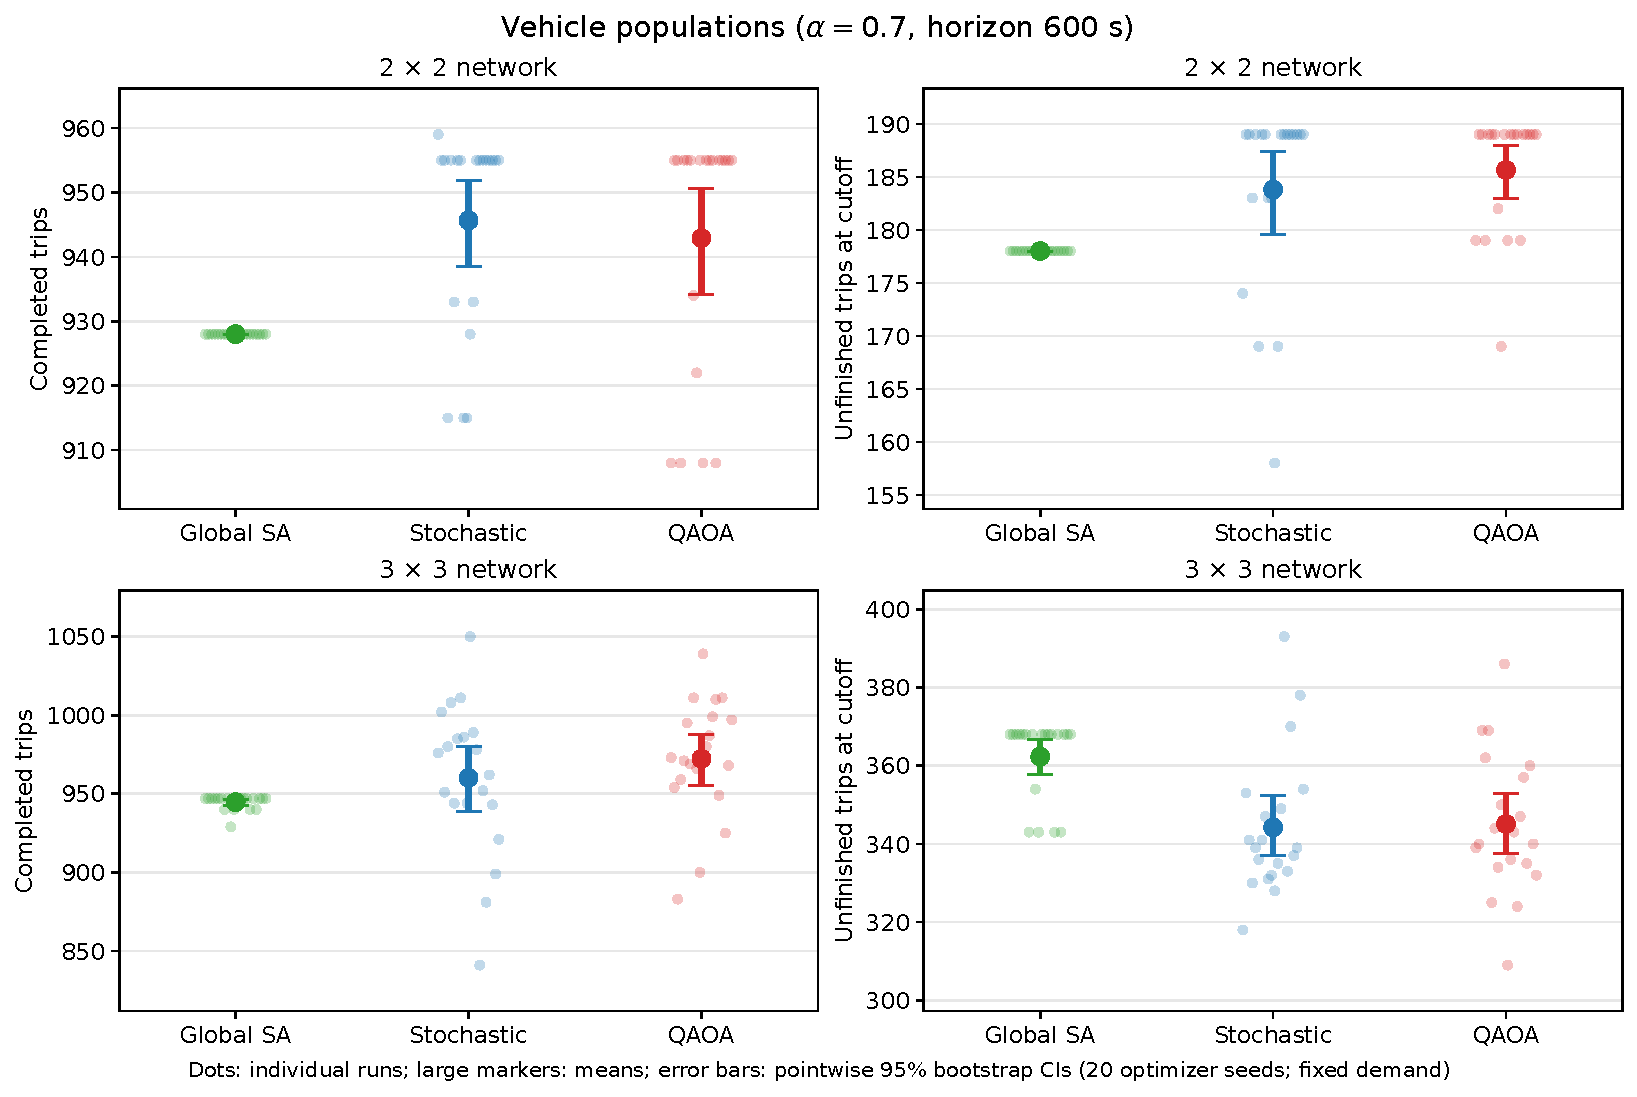
\includegraphics[width=\linewidth]{figure_population.pdf}
\caption{Completed and unfinished vehicle populations at the 600-s cutoff. All conditions use $\alpha=0.7$ and fixed demand. Small dots show individual optimizer runs; large markers show means and error bars show pointwise 95\% percentile-bootstrap confidence intervals across 20 optimizer runs. These are not confidence intervals for controller differences.}
\label{fig:supplementary-population}
\end{figure}

\begin{figure}[tbp]
\centering
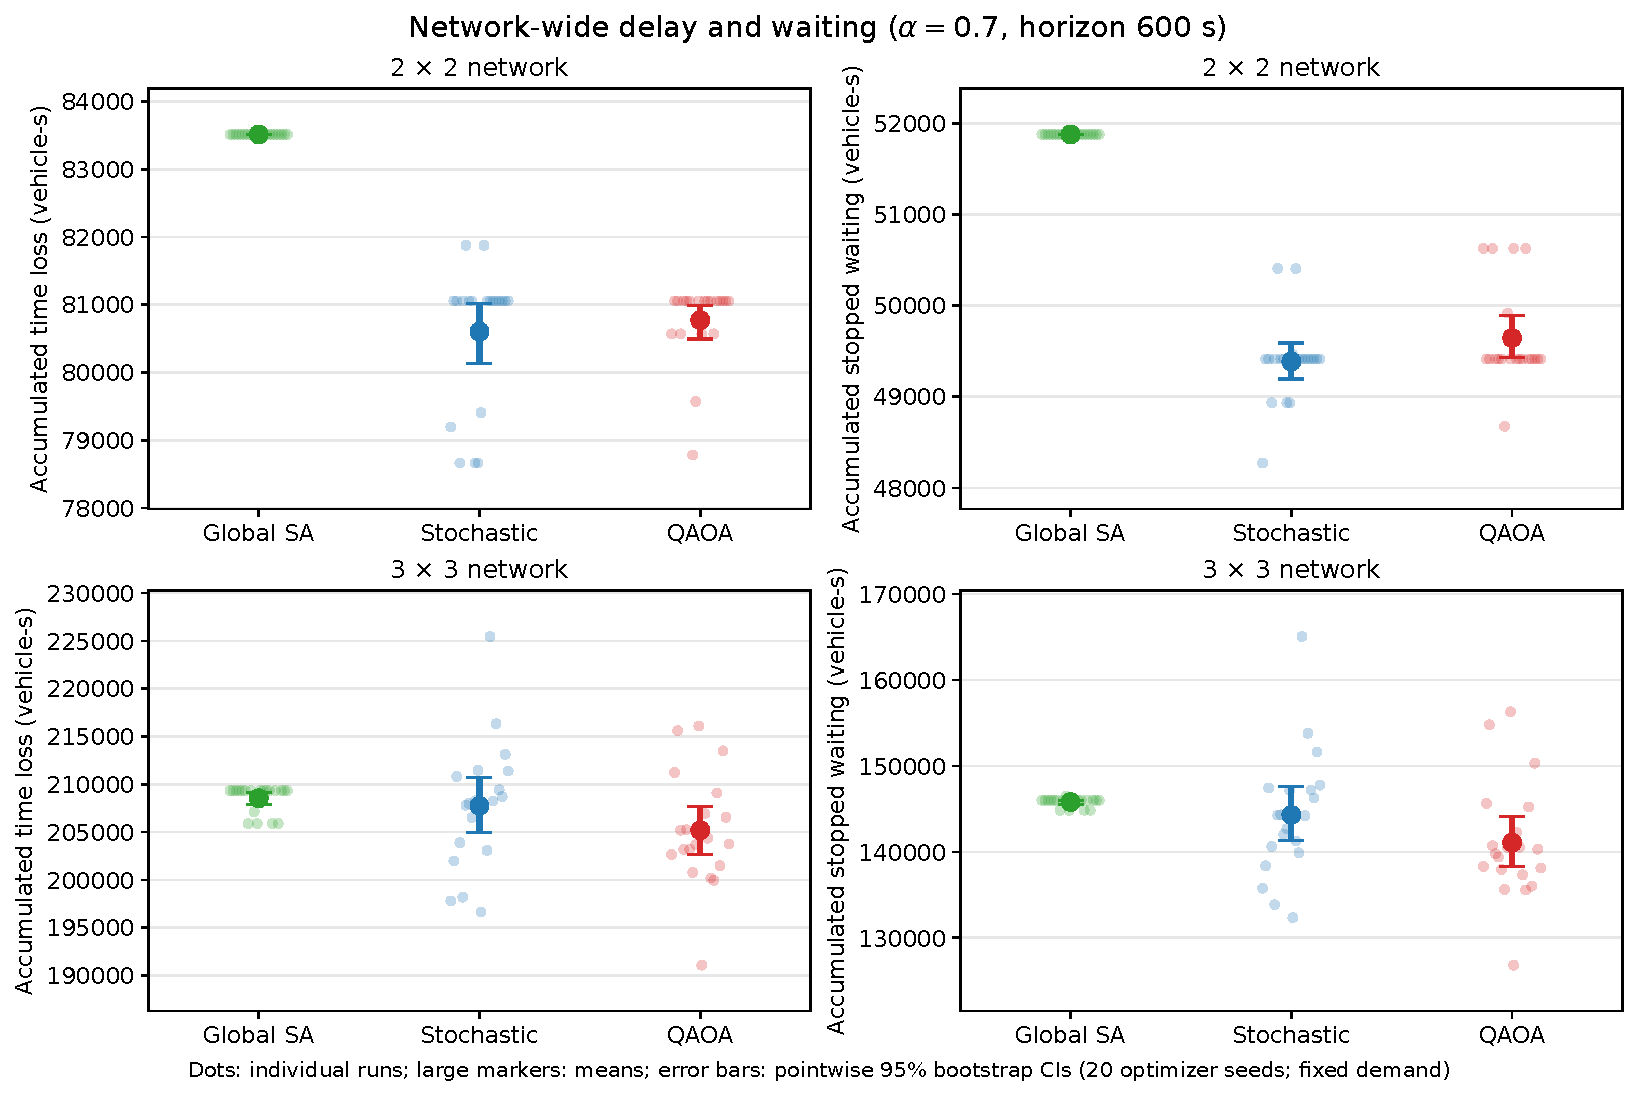
\includegraphics[width=\linewidth]{figure_network_delay.pdf}
\caption{Accumulated network-wide time loss and stopped waiting, including completed, unfinished, and any removed vehicles through the cutoff. Vehicles awaiting insertion are excluded and reported separately. All conditions use $\alpha=0.7$ and fixed demand. Small dots show individual optimizer runs; large markers show means and error bars show pointwise 95\% percentile-bootstrap confidence intervals across 20 optimizer runs. These are not confidence intervals for controller differences.}
\label{fig:supplementary-network-delay}
\end{figure}

\begin{figure}[tbp]
\centering
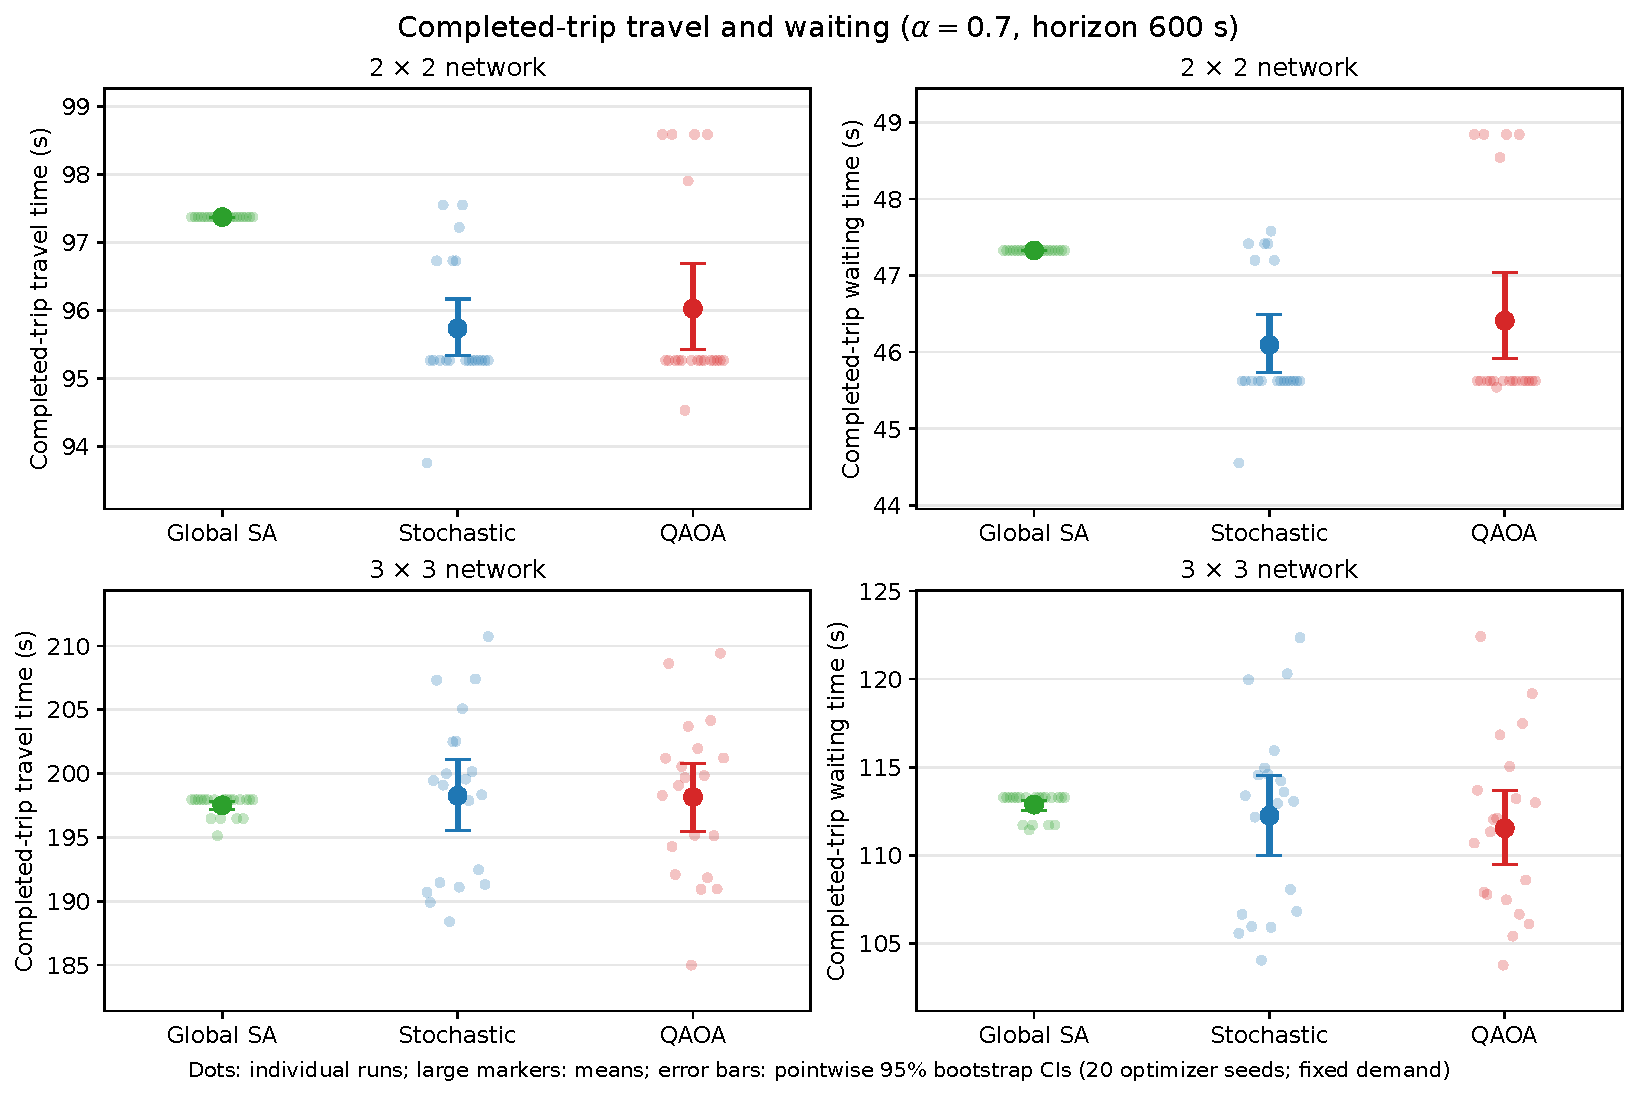
\includegraphics[width=\linewidth]{figure_trip_times.pdf}
\caption{Completed-trip travel and waiting times. These averages are interpreted alongside population and network-wide delay accounting. All conditions use $\alpha=0.7$ and fixed demand. Small dots show individual optimizer runs; large markers show means and error bars show pointwise 95\% percentile-bootstrap confidence intervals across 20 optimizer runs. These are not confidence intervals for controller differences.}
\label{fig:supplementary-trip-times}
\end{figure}

\begin{figure}[tbp]
\centering
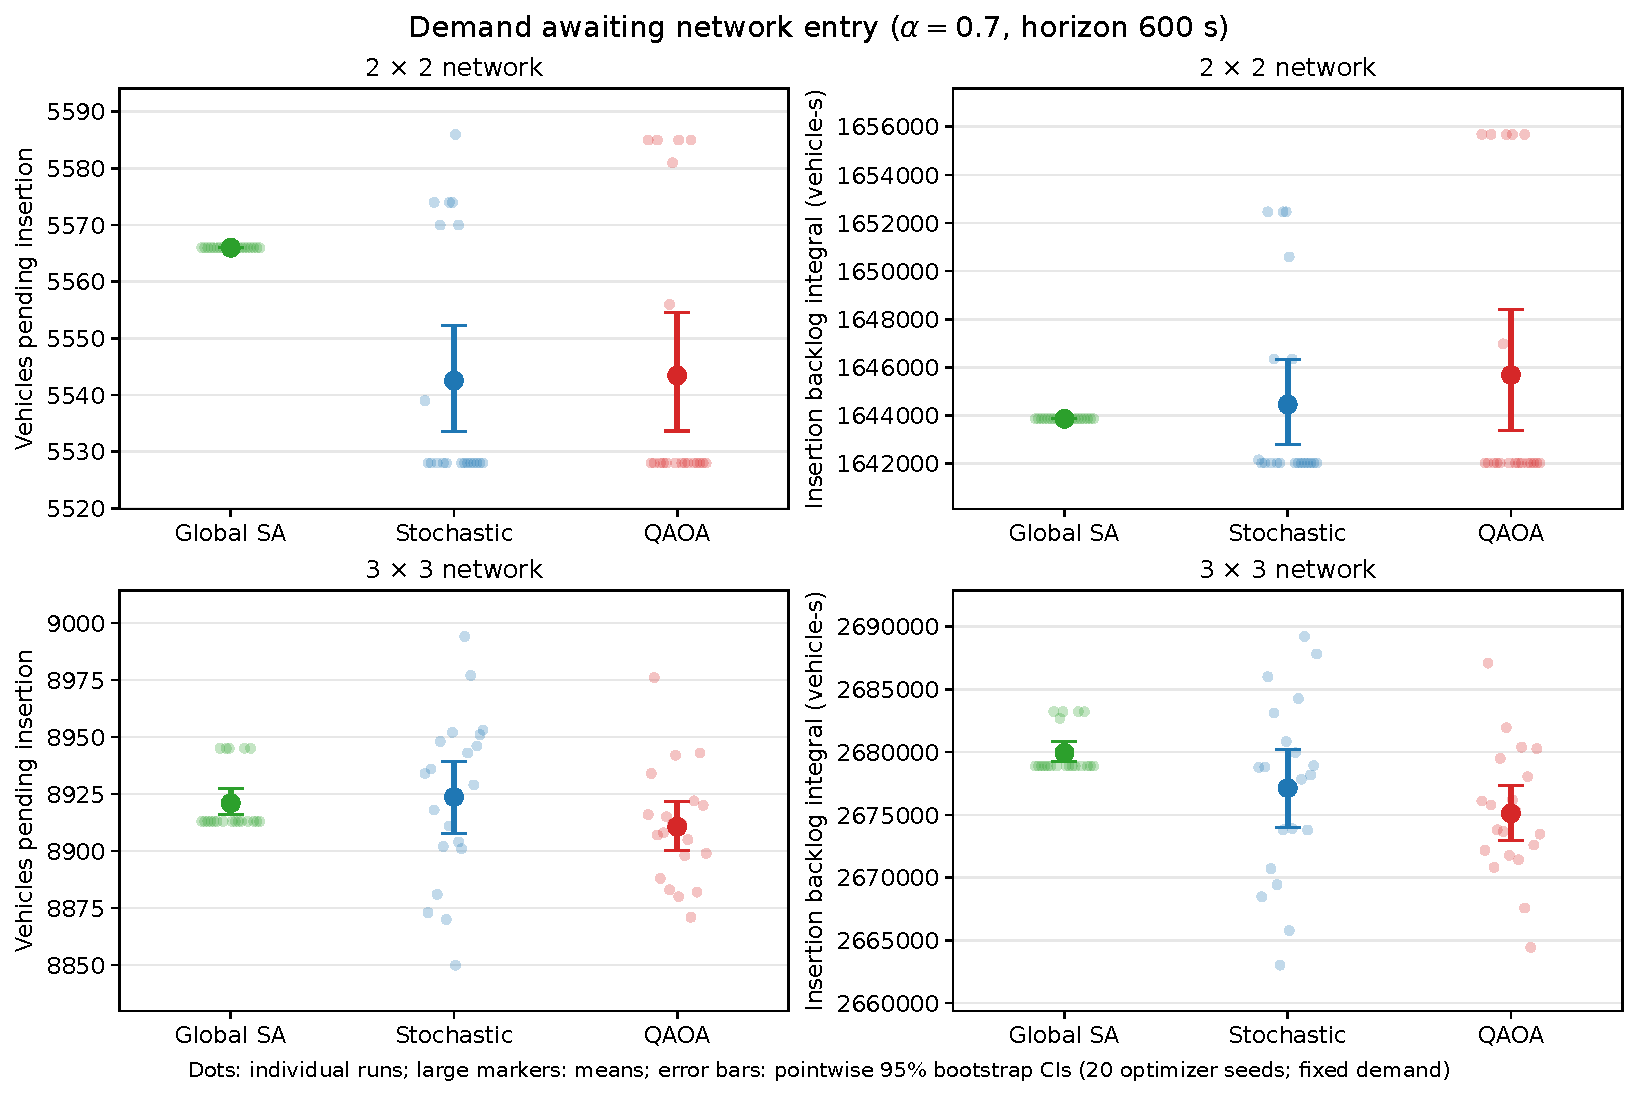
\includegraphics[width=\linewidth]{figure_insertion_backlog.pdf}
\caption{Vehicles pending insertion at the cutoff and accumulated insertion backlog, measured as a discrete right-endpoint integral. These quantities are separate from in-network time loss. All conditions use $\alpha=0.7$ and fixed demand. Small dots show individual optimizer runs; large markers show means and error bars show pointwise 95\% percentile-bootstrap confidence intervals across 20 optimizer runs. These are not confidence intervals for controller differences.}
\label{fig:supplementary-insertion-backlog}
\end{figure}


\begin{figure}[tbp]
\centering
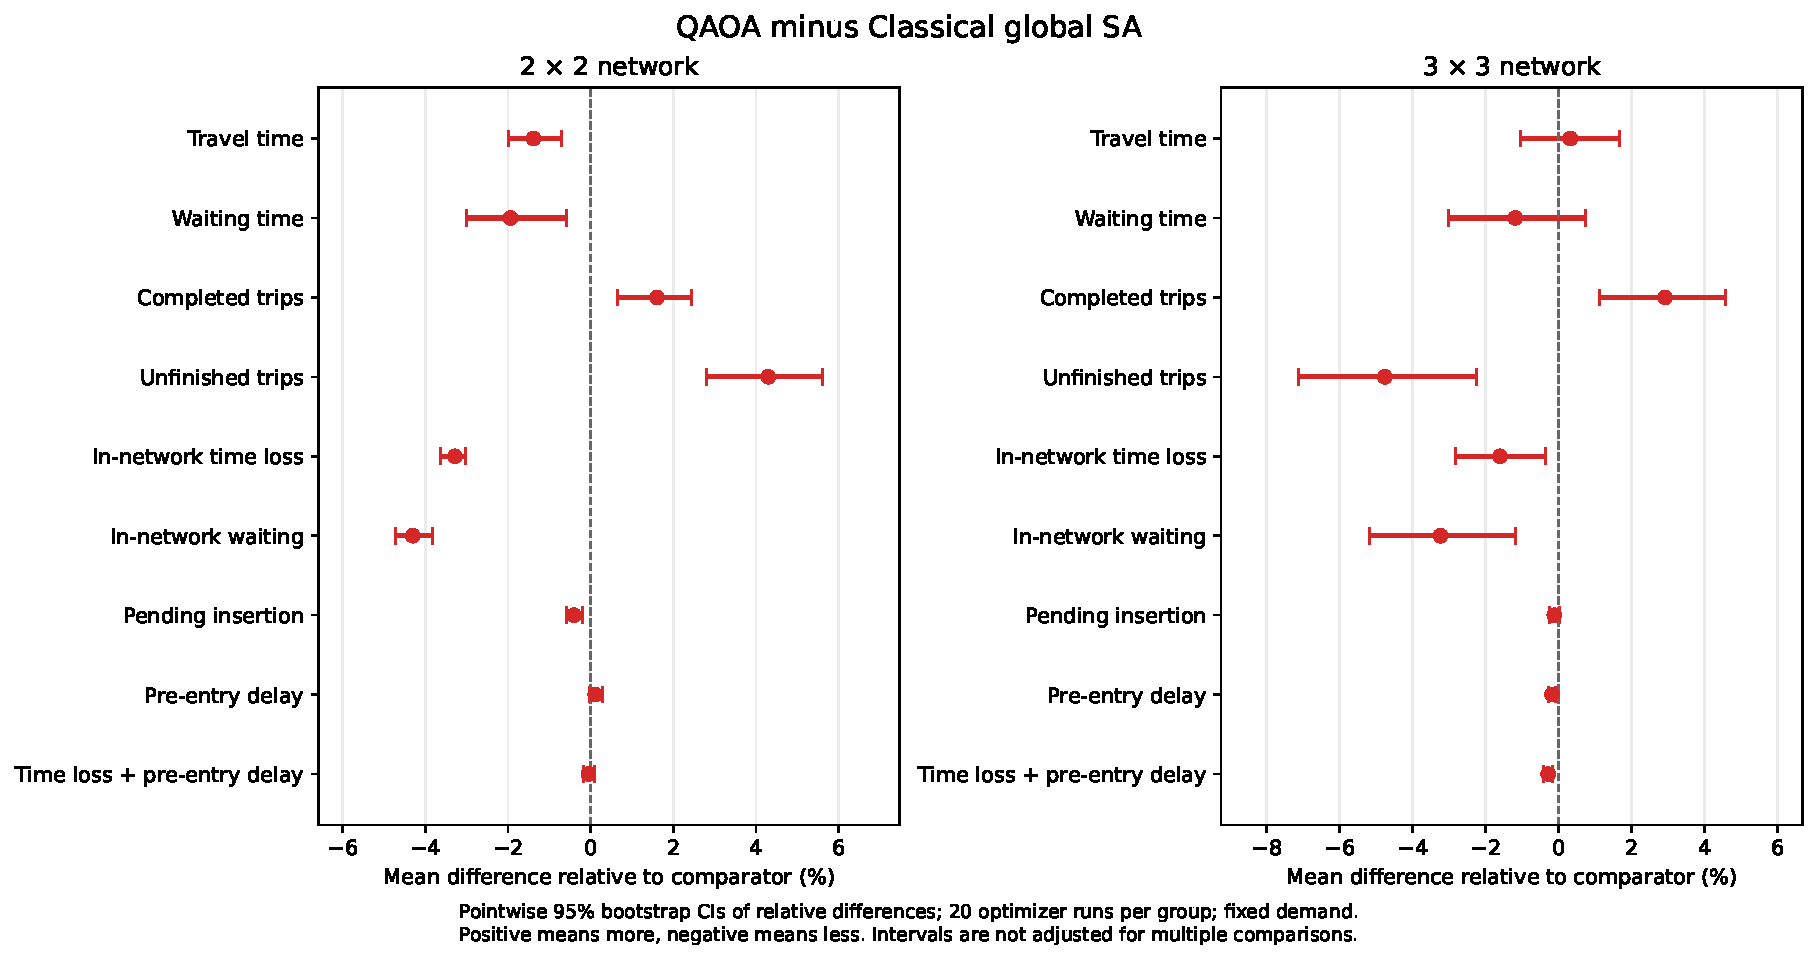
\includegraphics[width=\linewidth]{figure_effects_qaoa_vs_global.pdf}
\caption{QAOA minus global SA: relative mean differences with pointwise 95\% independent run-level bootstrap confidence intervals. Positive values mean more and negative values mean less; larger completed counts are favorable, while smaller travel, waiting and delay values are favorable. Intervals are not multiplicity-adjusted; corresponding Welch and Holm-adjusted tests are reported in the statistical tables. All traffic results use fixed demand, $\alpha=0.7$ and a 600-s cutoff; uncertainty concerns optimizer randomness, not traffic-demand scenarios.}
\label{fig:revised-effects-qaoa-vs-global}
\end{figure}

\begin{figure}[tbp]
\centering
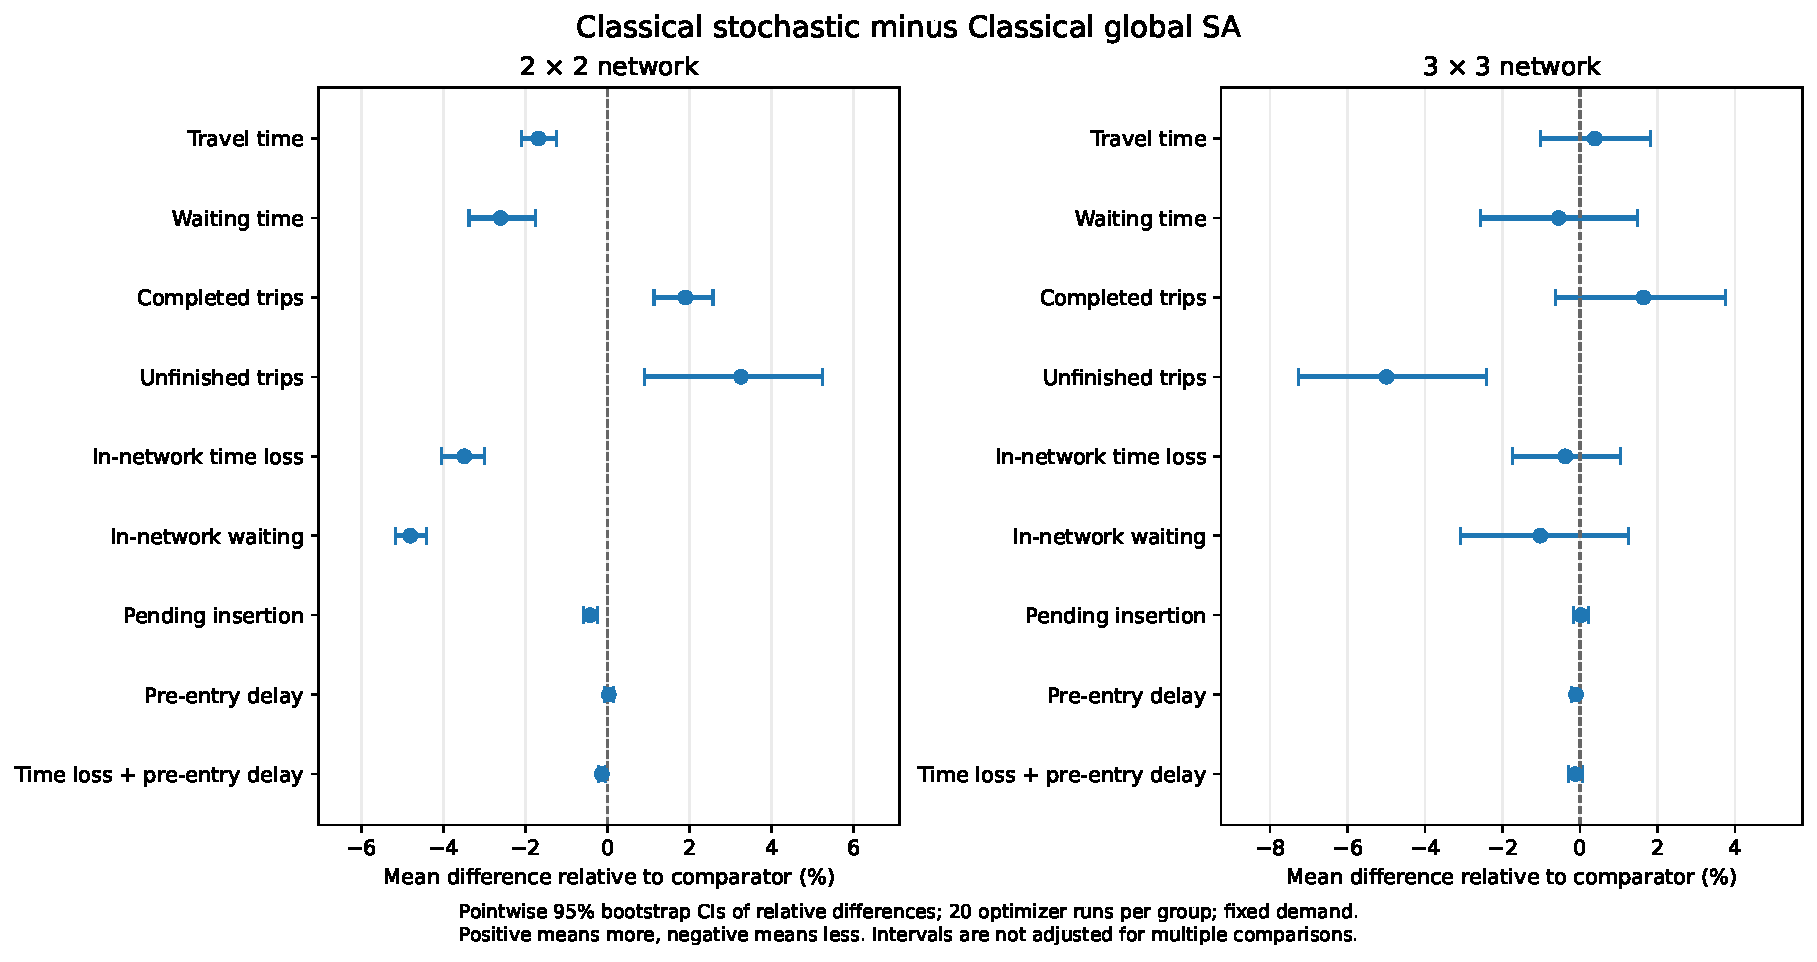
\includegraphics[width=\linewidth]{figure_effects_stochastic_vs_global.pdf}
\caption{Classical stochastic minus global SA: relative mean differences with pointwise 95\% independent run-level bootstrap confidence intervals. Intervals are not multiplicity-adjusted; see the adjusted-effects tables. All traffic results use fixed demand, $\alpha=0.7$ and a 600-s cutoff; uncertainty concerns optimizer randomness, not traffic-demand scenarios.}
\label{fig:revised-effects-stochastic-vs-global}
\end{figure}

\begin{figure}[tbp]
\centering
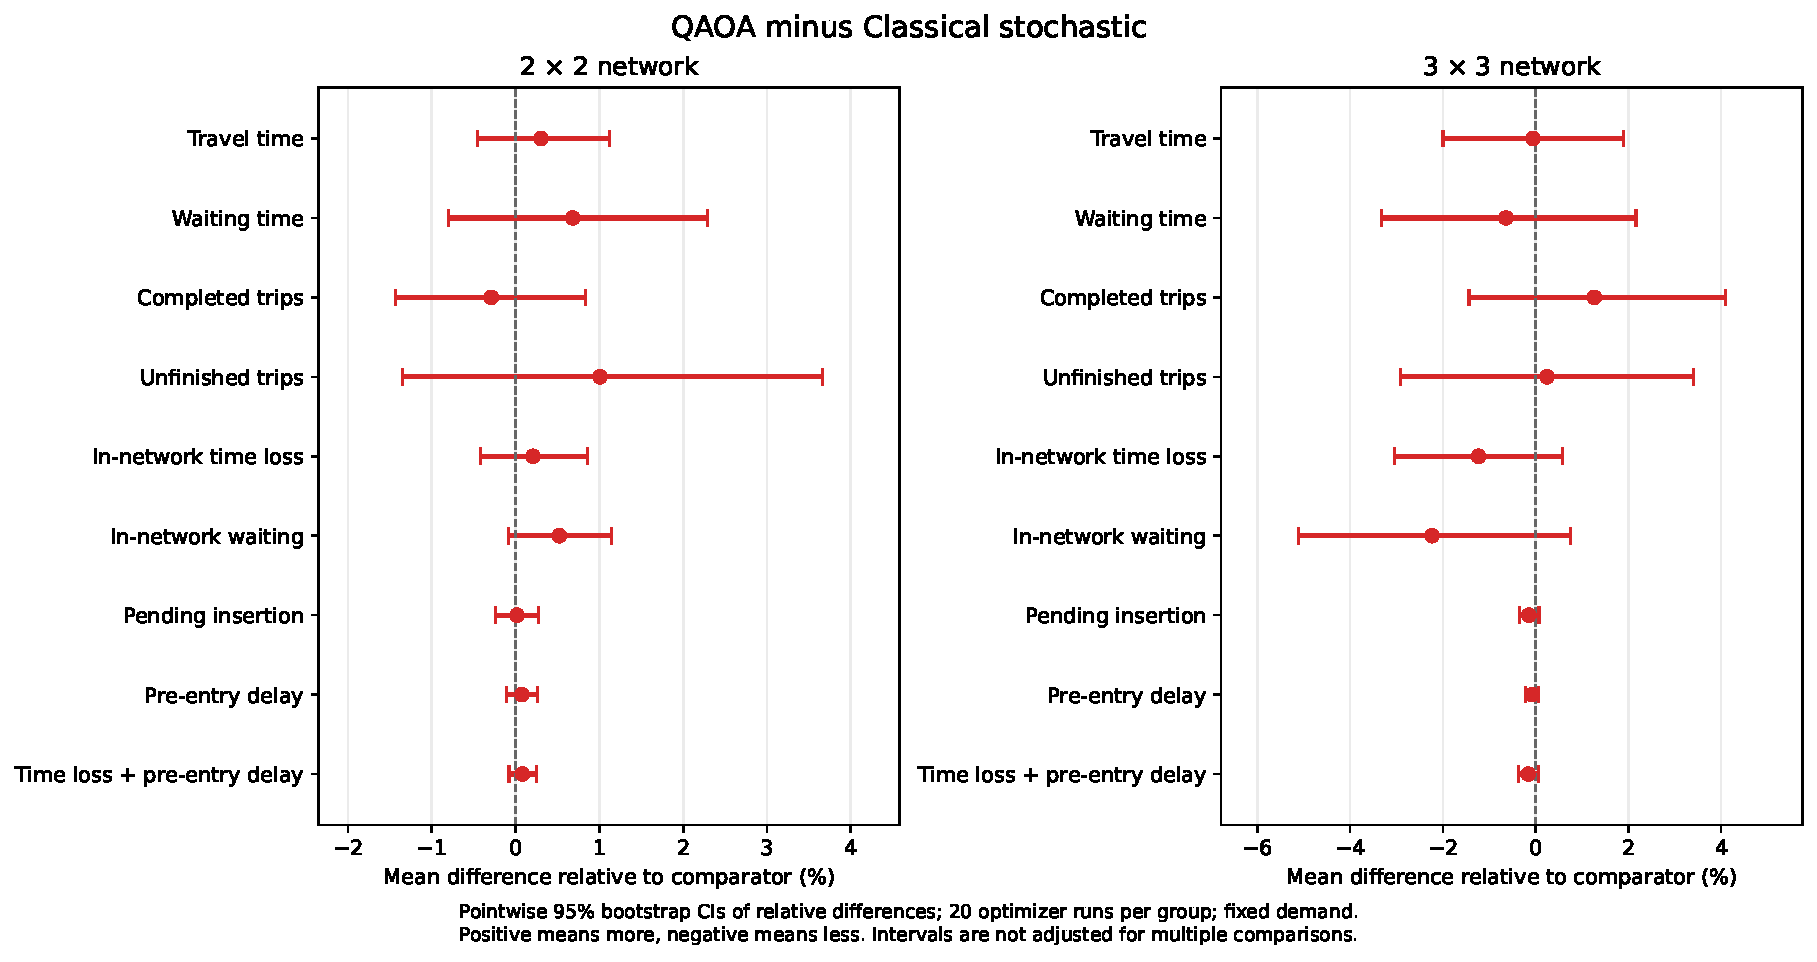
\includegraphics[width=\linewidth]{figure_effects_qaoa_vs_stochastic.pdf}
\caption{QAOA minus classical stochastic: relative mean differences with pointwise 95\% independent run-level bootstrap confidence intervals. Intervals spanning zero do not establish equivalence. Corresponding multiplicity-adjusted tests are reported separately. All traffic results use fixed demand, $\alpha=0.7$ and a 600-s cutoff; uncertainty concerns optimizer randomness, not traffic-demand scenarios.}
\label{fig:revised-effects-qaoa-vs-stochastic}
\end{figure}

\begin{figure}[tbp]
\centering
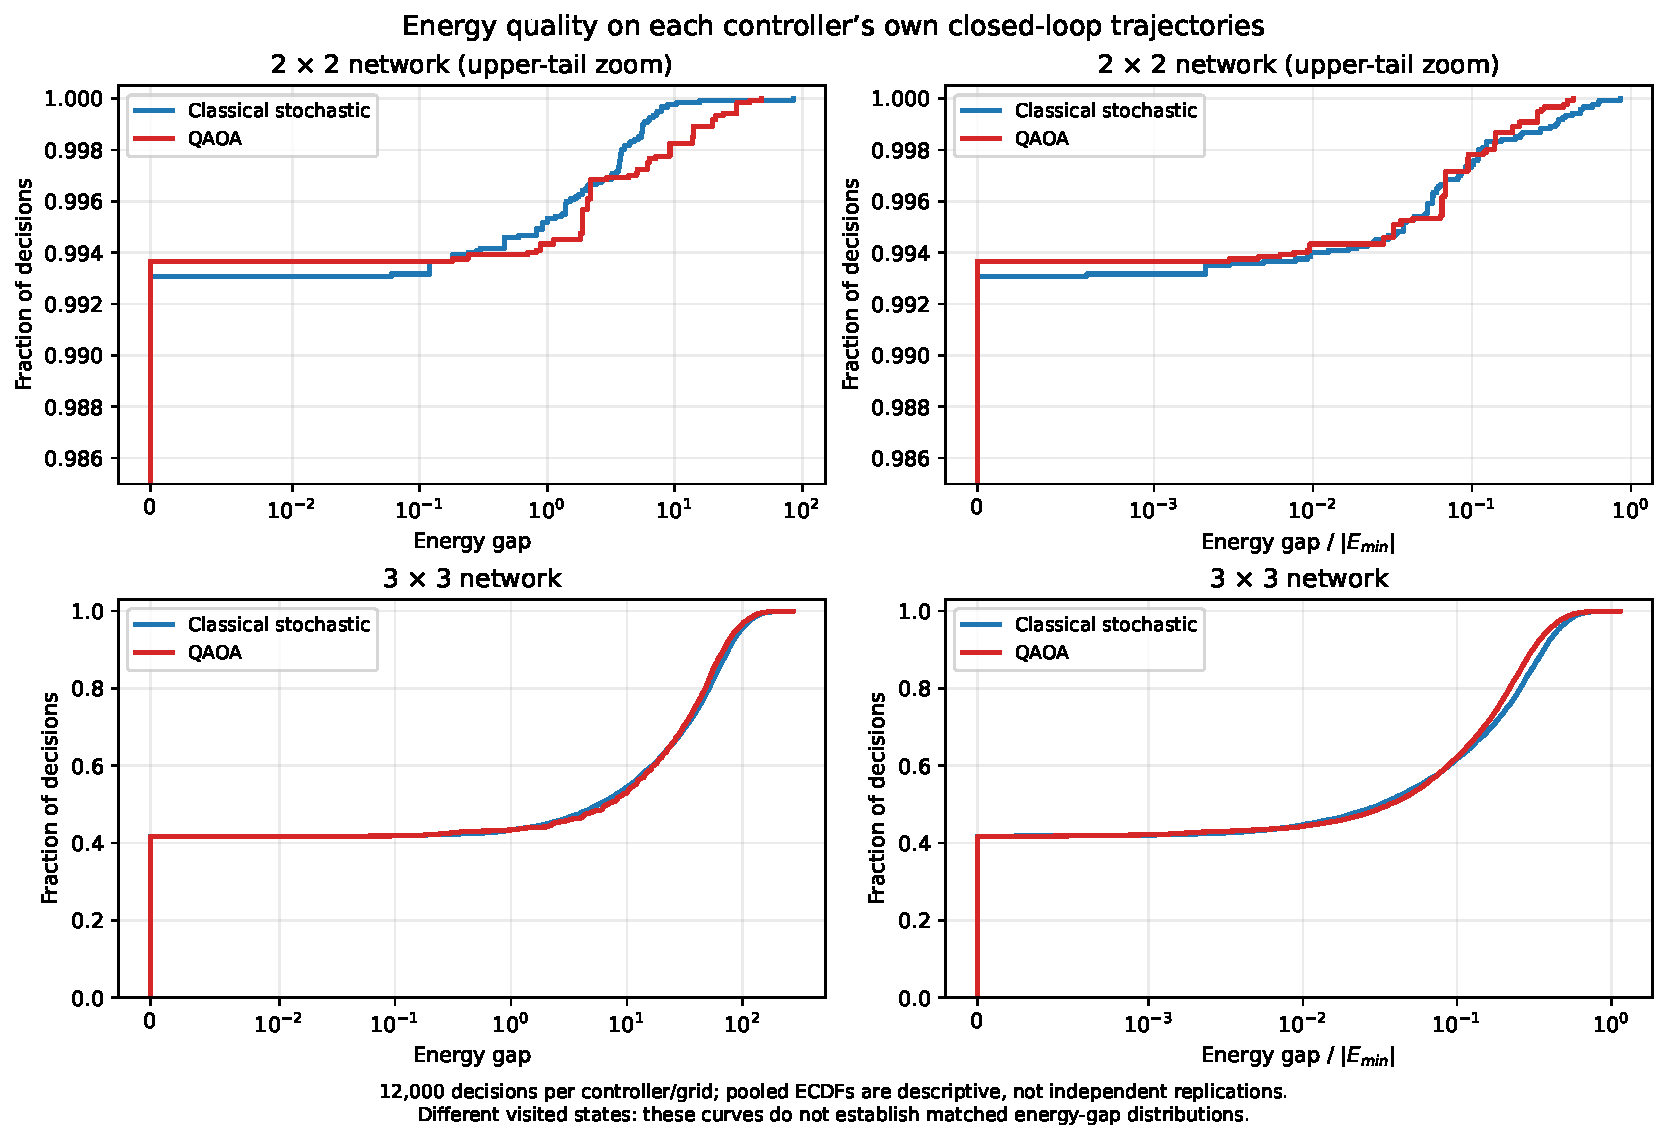
\includegraphics[width=\linewidth]{figure_energy_gaps.pdf}
\caption{Raw and normalized energy-gap ECDFs along each controller\textquotesingle s own closed-loop trajectories. Normalization divides each gap by the absolute exact minimum energy for that decision (nonzero for all retained decisions). The symmetric-log horizontal scales preserve zero and display positive tails. The 2x2 panels zoom to ECDF values above 0.985 because almost all decisions recover the optimum. Pooled decisions are descriptive and not independent replications. These trajectories visit different Hamiltonians, so visual similarity does not certify distribution matching; saved common-state diagnostics are reported separately. All traffic results use fixed demand, $\alpha=0.7$ and a 600-s cutoff; uncertainty concerns optimizer randomness, not traffic-demand scenarios.}
\label{fig:revised-energy-gaps}
\end{figure}

\begin{figure}[tbp]
\centering
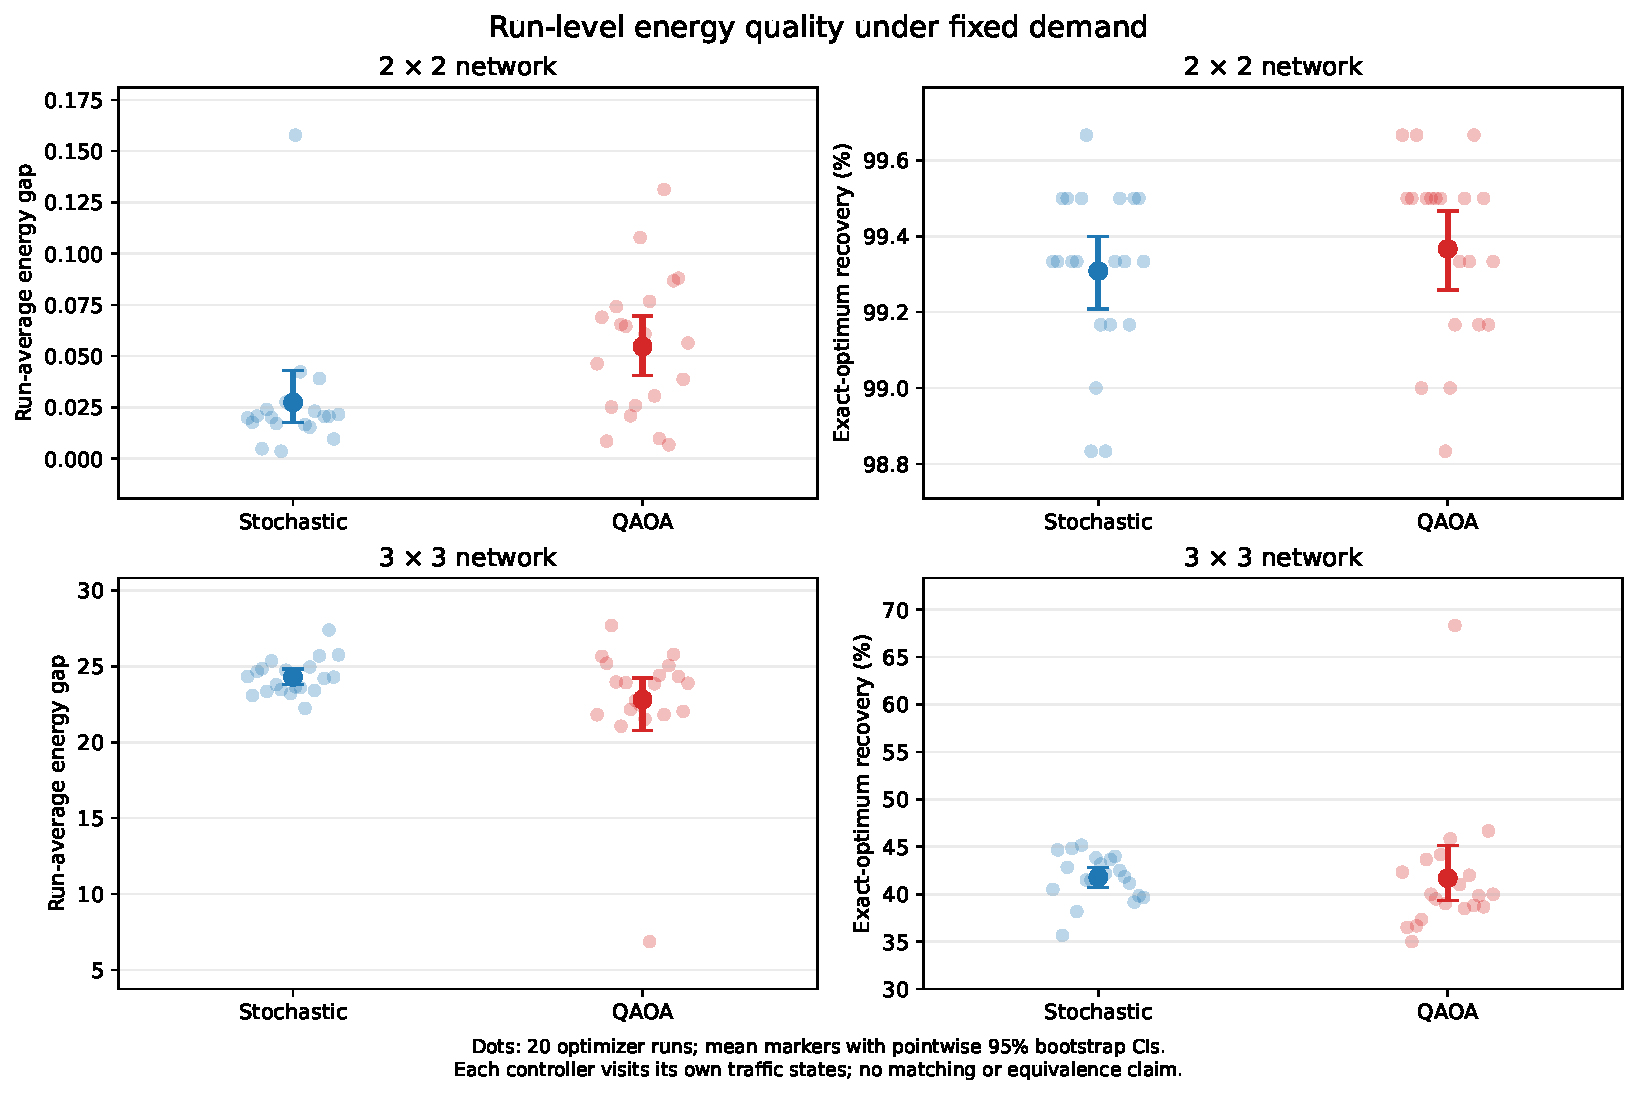
\includegraphics[width=\linewidth]{figure_energy_run_summary.pdf}
\caption{Run-level mean energy gaps and exact-optimum recovery on the controllers\textquotesingle{} respective traffic trajectories. Small dots represent individual runs; large markers and bars show means and pointwise 95\% bootstrap confidence intervals across 20 runs. All traffic results use fixed demand, $\alpha=0.7$ and a 600-s cutoff; uncertainty concerns optimizer randomness, not traffic-demand scenarios.}
\label{fig:revised-energy-run-summary}
\end{figure}

\begin{figure}[tbp]
\centering
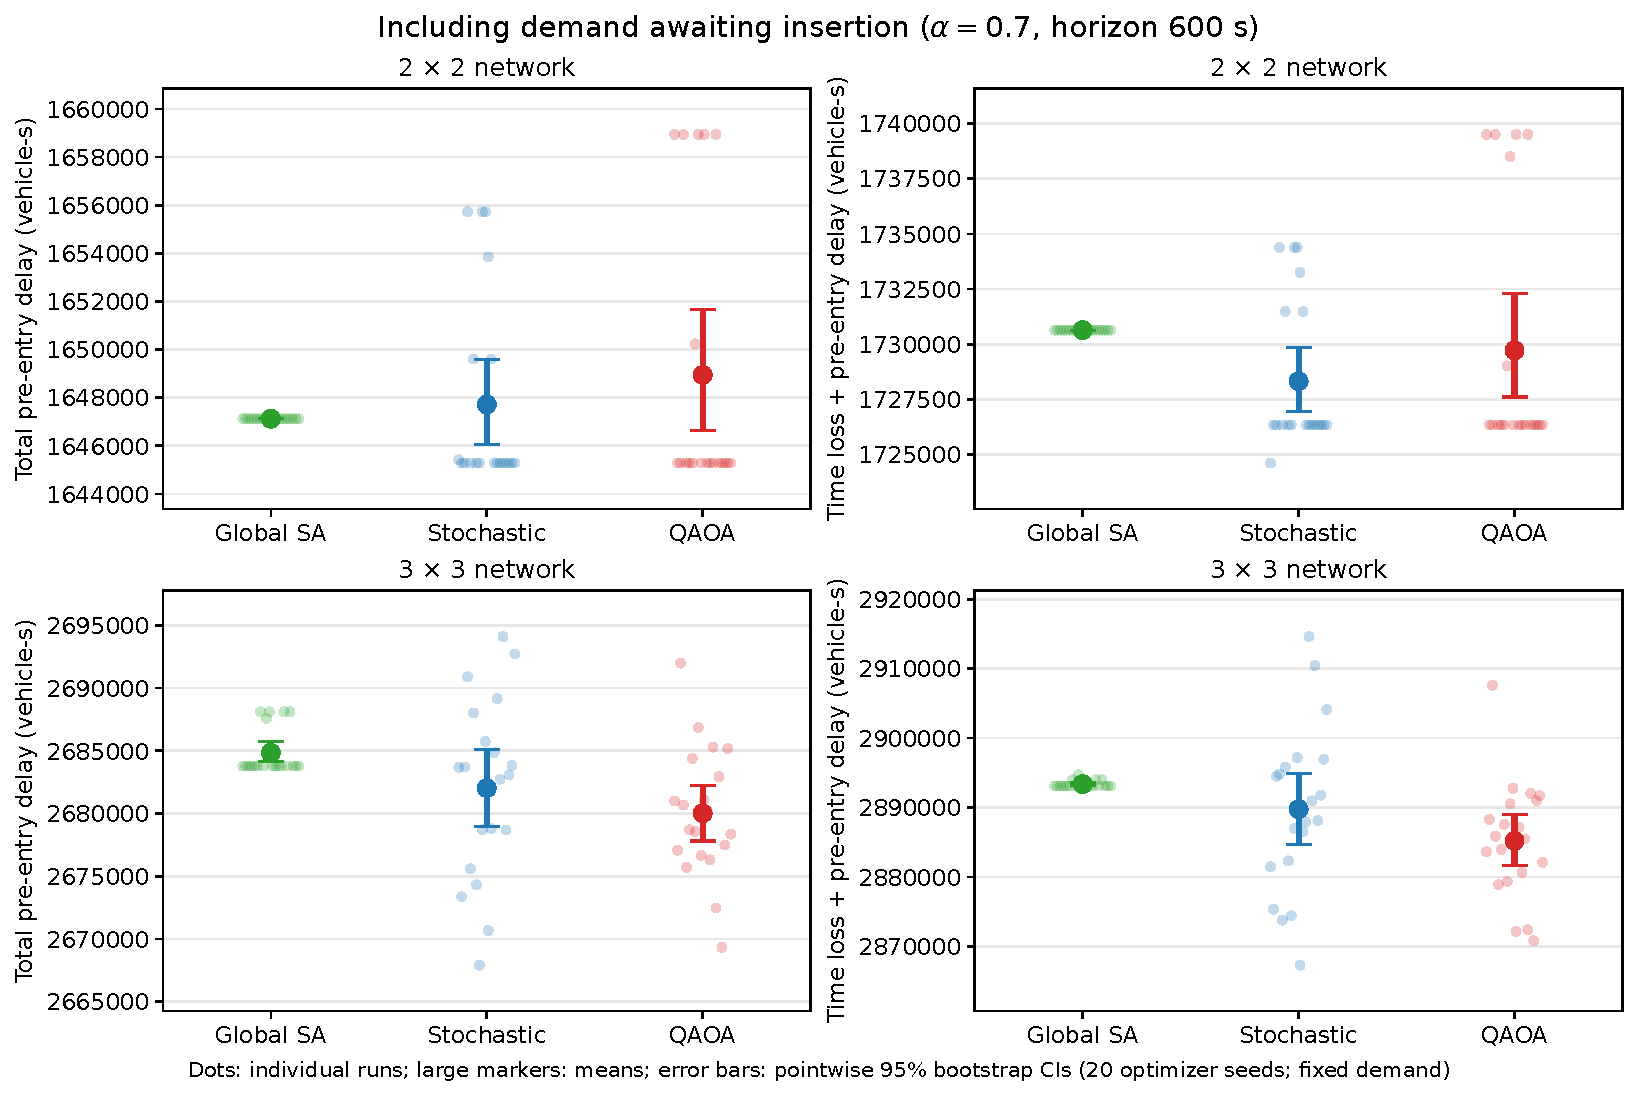
\includegraphics[width=\linewidth]{figure_total_delay.pdf}
\caption{Pre-entry delay and the supplementary sum of in-network time loss plus pre-entry delay. Pre-entry delay sums the SUMO departDelay field across entered and undeparted vehicles through the cutoff. The sum joins disjoint pre-entry and in-network phases. It does not add stopped waiting to time loss or add the sampled backlog integral again. Small dots show runs; mean markers have pointwise 95\% bootstrap confidence intervals. All traffic results use fixed demand, $\alpha=0.7$ and a 600-s cutoff; uncertainty concerns optimizer randomness, not traffic-demand scenarios.}
\label{fig:revised-total-delay}
\end{figure}

\end{document}